\documentclass[12pt, a4paper]{report}
\usepackage[margin = 1.5in]{geometry}
\usepackage{hyperref}
\usepackage{xr-hyper}
\usepackage{graphicx}
\graphicspath{ {./images/}{./figures} }
\usepackage{setspace} %For title page spacing
\usepackage{algorithm, algpseudocode}
\usepackage{amsthm} %For proofs
\usepackage{tikz} %For diagrams
\usepackage{standalone} %So that diagrams can be standalone figures

% Spacing modification between paragraphics
\usepackage{parskip}
\parskip=12pt
% Removes extra parskip added before proofs to make spacing better
\AtBeginEnvironment{proof}{\vspace*{-\parskip}}

\usepackage{caption}
\captionsetup{justification=centering}

% Bibliography styling
\usepackage[
    backend=biber,
    style=ieee,
    sorting=nty
    ]{biblatex}
\addbibresource{bibliography.bib}
\setlength{\bibitemsep}{0.5\baselineskip}

% Command to draw any number of a certain input character (useful for typing Dyck words)
\makeatletter
\newcount\char@repeat@count
\newcommand{\charrepeat}[2]{%
  \begingroup
  \char@repeat@count=\z@
  \@whilenum\char@repeat@count<#1\do{\texttt{#2}\advance\char@repeat@count\@ne}%
  \endgroup
}
\makeatother

% \usepackage{newunicodechar}
% % Command to define £ as a delimiter for \texttt
% \newunicodechar{§}{\makeabbreviationtt}
% \def\makeabbreviationtt#1§{\texttt{#1}}

% Command for big O notation symbol
\newcommand{\bigO}{\mathcal{O}}

% Definining the types of theorems we can have, and ensuring they can be referenced to correctly later with hyperlinks
\newtheorem{definition}{Definition}
\newcommand{\definitionautorefname}{Definition}
\newtheorem{theorem}{Theorem}
% \newcommand{\theoremautorefname}{Theorem}
\newtheorem{observation}{Observation}
\newcommand{\observationautorefname}{Observation}
\newtheorem{claim}{Claim}
\newcommand{\claimautorefname}{Claim}

\begin{document}


\thispagestyle{empty}

\vspace*{\fill}
\begin{spacing}{2}
    \begin{center}
        
\includegraphics[scale = 0.45]{WarwickCrest.pdf}
    \end{center}
    \vspace{5mm}
    \begin{center}
        \textbf{\LARGE An analysis of strategies in the re-pairing game}
  
		\vspace{5mm}
	\end{center}
	\begin{center}
		{\large CS344 Discrete Mathematics Project}\\
	\end{center}
	\begin{center}
        \vspace{20mm}
		\textbf{\large Laveen Chandnani}
		\vspace{20mm}
	\end{center}
	\begin{center}
	     {\large Supervisors: Dr. Dmitry Chistikov \& Dr. Matthias Englert }\\
		\textbf{\large Department of Computer Science}\\
	\end{center}
    
\end{spacing}
\vspace*{\fill}
\clearpage
\thispagestyle{empty}
\nointerlineskip
\vspace*{\fill}
    
\section*{\center \abstractname}
The project expands on the work of Chistikov and Vyali, which introduced a simple one-player game; The re-pairing game can be played on any well-formed sequence of opening and closing brackets (a Dyck word). A move consists of "pairing" any opening bracket with any closing bracket to the right of it, and "erasing" the two. The process is repeated until we are left with no remaining brackets. Such a game can have many strategies, but the effectiveness of a strategy is measured by it's width, which is the maximum number of nonempty segments of symbols seen during a play of the game.

\textbf{Keywords:} \textit{Dyck language, Re-pairing brackets, Combinatorics, Web application, Python, ReactJS}

\section*{\center Acknowledgements}
I'd like to thank my dissertation supervisors, Dr. Dmitry Chistikov and Dr. Matthias Englert, for their invaluable guidance, support and feedback throughout this project. 

I'd also like to thank Melany Henot, Varshneyan Prabakaran, Brendan Bell, Raumaan Ahmed, Varun Chodanker and Devon Connor for engaging in insightful discussions on some of the problems I tackled, and for their continued support which enabled me to complete this project throughout a difficult year.

\vspace*{\fill}

\tableofcontents

\pagenumbering{arabic}
\section{Introduction}

We start with a simple one-player game. Take any Dyck word (a balanced sequence of opening and closing brackets), for example:

\null
\begin{center}
    \texttt{\large (()())}
\end{center}
\null

\noindent A move in this game consists of pairing any opening bracket with any closing bracket to its right, and replacing the two with a blank space, denoted with the \texttt{\string_} symbol. This process is repeated until there are no more brackets to pair up, resulting in the empty string, and the sequence of moves made is called a re-pairing. An example of a re-pairing is as follows:

\null
\begin{center}
    \texttt{\large (()())}\\
    \texttt{\large (\string_)(\string_)}\\
    \texttt{\large \string_\string_\string_(\string_)}\\
    \texttt{\large \string_\string_\string_\string_\string_\string_}\\
\end{center}
\null

\noindent Note that our first move pairs up two brackets that are not matched to each other in the initial word. We allow such moves in a re-pairing. 

Finding any re-pairing following these rules is a trivial task, but we want to measure how good a re-pairing is. For this we introduce a property called the width, defined as the maximum number of non-empty segments of brackets seen during the re-pairing. We can see that the previous re-pairing had width 2. A natural question then arises; can we obtain a re-pairing with a smaller width? The answer for this particular string is yes, and such a re-pairing is shown below:

\null
\begin{center}
    \texttt{\large (()())}\\
    \texttt{\large \string_()()\string_}\\
    \texttt{\large \string_()\string_\string_\string_}\\
    \texttt{\large \string_\string_\string_\string_\string_\string_}\\
\end{center}
\null

\noindent Here we see this re-pairing has width 1. Our goal is to try and minimise this width as much as possible. 


\subsection{Objectives}

This project aims to take both a theoretical and practical approach to this game. It aims to assess the current literature available on the game and expand on their results. This allows us to get a broader picture of the research landscape on the game, as well as a deeper and more intuitive grasp on certain results. The project also aims to implement these strategies in a practical way that allows for visualisation and experimentation. Finally, the project aims to attack the goal of minimising width with a practical approach, by analysing certain strategies and subcases of Dyck words. More specifically, the objectives of the project can be outlined as follows:

\begin{enumerate}
    \item An introduction to the relevant definitions and content to lay out relevant background knowledge.
    \item Expanding on and providing potential novel insights on well established results.
    \item Establishing the research landscape on the re-pairing game and relevant topics.
    \item Creating software to demonstrate re-pairing strategies from literature and allow manual experimentation on Dyck word re-pairings.
    \item Using software to analyse subcases of Dyck words and exhaustively find their width in an attempt to pin down the formula of a general Dyck word.
\end{enumerate}

\subsection{Related work}
This project builds on the work from Chistikov and Vyalyi \cite{chistikov2020re}, whose paper serves as a basis for this project. The paper introduces this game as a way to prove a lower bound on translating one-counter automata (OCA) into Parikh-equivalent nondeterministic finite automata (NFA). It provides lower bounds on the width for simple and non-simple re-pairings, which is then used to prove lower bounds on these translations.

Due to the specialised nature of this game's origins, there are no other works on this game at the time of writing.


\section{Literature Review}
\chapter{A web application for the game} This section discusses the process of implementing a web application that allows for visualisation and experimentation of the re-pairing game. 

\section{Software Requirements}
Before any software was written, a list of requirements for the software was made. These are features that the software must have in order to fulfill the relevant objectives, and were subsequently tested throughout the development of the web application:
\begin{enumerate}
    \item Allow a user to enter Dyck words.
    \item Validate a given input and provide a relevant error message if required.
    \item Display the given Dyck word with the ability for manual interaction via a mouse.
    \item Verify that the characters selected are a valid move before allowing them to be paired.
    \item Allow for the use of strategies from literature (Simple, Non-Simple recursive), as well as our own strategies (Simple Greedy, Brute Force).
    \item If selecting a strategy, generate a list of moves before visualising the play.
    \item Display the list of moves, and allow the user to jump to any move in the play.
    \item Display a running width counter from the moves seen so far, and the width of the overall play if a strategy has been used.
    % \item (OPTIONAL) Allow for a mix between manual re-pairing and the use of pre-defined strategies (e.g. re-pairing the first half of a word using a strategy, and completing the second half using manual selections).
    \item Allow the user to brute force a given list of Dyck Words, and return the optimal widths of each along with the re-pairing.
\end{enumerate}

\section{Technologies}
The development of the web application went through multiple iterations before settling on the current choice of technologies used. The application uses the JavaScript library React for the frontend user interface with the Material UI library for components, and the Python web framework Flask for the backend algorithms with PyPy for faster runtimes. This section discusses the decisions made when choosing the main technologies (frameworks, libraries etc).

\subsection{Initial Ideas}
 The software was initially planned to be a local Python only application, using the Tkinter GUI library. This was because the author is most familiar with the Python programming language, and has some limited experience with the Tkinter library. However, early prototypes of this software using Tkinter proved to be cumbersome to work with and have a dated visual style. Alternative Python UI libraries (such as PyQt and Kivy) were also considered, but proved to have learning curves no steeper than using an entirely different language.
\begin{figure}[H]
    \centering
    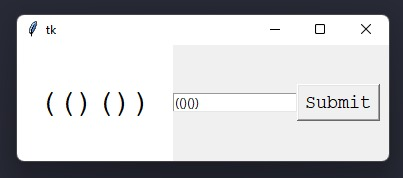
\includegraphics[scale = 0.7]{./images/tkinter-gui.jpeg}
    \caption{An early iteration of the software using Tkinter}
\end{figure}
\noindent We then considered the prospect of a web application; the author again had some limited experience with HTML/CSS, but using these languages to control the layout and sizing of the UI seemed much more intuitive. This approach also naturally allowed for separation between the UI and the strategies, and the author's familiarity with Python could still be leveraged as a backend language. The author had also wished to learn the technologies used for web development, so this seemed like the natural approach to take.

\subsection{Backend}
The strategies to run on Dyck words are implemented in Python but run using PyPy, and communicated with the frontend using Flask.

\subsubsection{Flask}
Flask is a web framework that allows users to build a web server with Python that they can communicate with using HTTP requests, allowing Python to be used as a backend language \cite{whatisFlask}. One of the reasons Flask was chosen over potential alternatives, such as Django, is due to its simplicity. Flask is classed as a microframework, meaning it does not have a lot of dependencies or libraries required to use it. This makes Flask fairly lightweight and efficient for our purposes, reducing overhead when communicating requests back and forth. 

\begin{figure}[H]
    \centering
    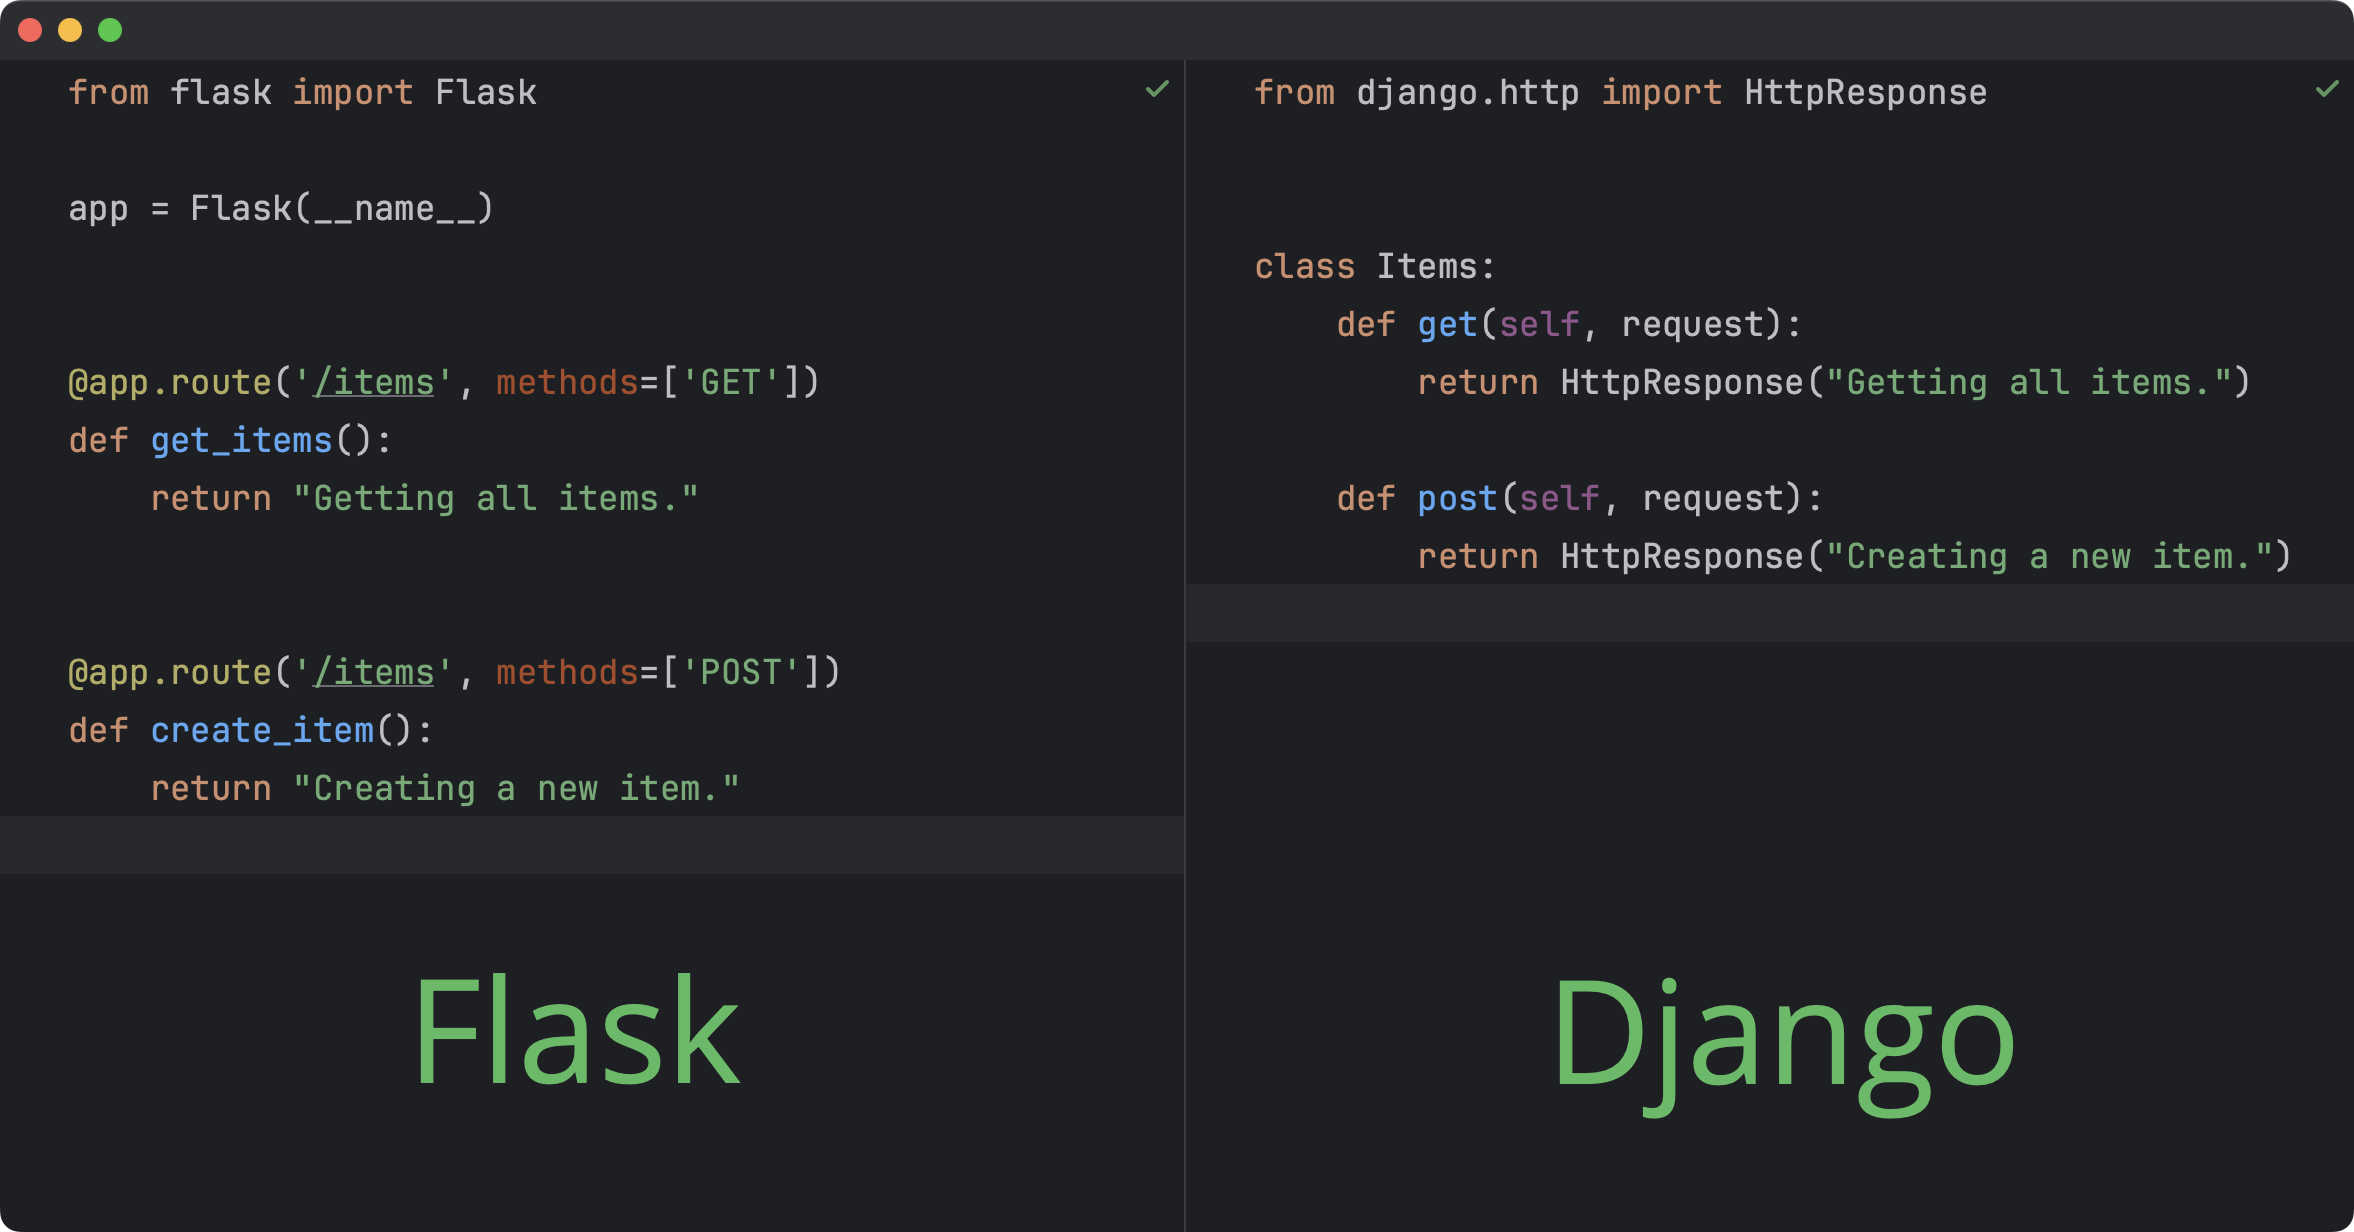
\includegraphics[scale=0.3]{./images/flaskVSdjango.png}
    \caption{Implementing the same functionality in Flask and Django \cite{flaskVSdjango}}
\end{figure}

\noindent Figure 3.2 shows the difference between using Flask and Django. In the Flask example, the same functions could be used with the only modification being an app route, which is added directly above the function. This binds each function to the route URL plus its given route, and depending on the type of request either ``get\textunderscore~items()'' or ``create\textunderscore~items()'' would be called. Thus, any work done to translate a re-pairing strategy into an algorithm could easily be implemented using Flask by simply adding an app route at the top.

\subsubsection{PyPy}
During the implementation of the web application, the author discovered PyPy. This is an alternative implementation of Python, providing faster execution times and less memory usage than the standard implementation.

\par\null\par
\noindent In particular, PyPy uses a Just-In-Time compiler, which converts Python code into machine code at runtime. This makes PyPy have the greatest speed-up when executing long-running programs where a significant fraction of the time is spent executing Python code \cite{whatisPyPy}, which is exactly what the backend will be doing (particularly when brute forcing for the width of a Dyck word). 

\par\null\par
\noindent Exceution of the program below, which computes the factorial of 20000 and repeats this 500 times, demonstrates the potential speed-up that PyPy can provide:

\begin{figure}[H]
    \centering
    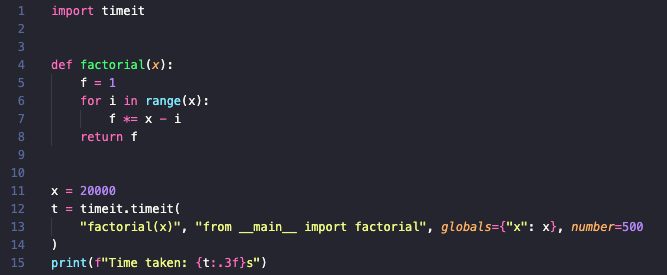
\includegraphics[scale=0.55]{./images/factorialPyPy.png}
    \caption{Computes 20000! 500 times}
\end{figure}

\noindent Executing this program using Python takes 77.930s, but using PyPy takes 31.872s. The program also requires no modifications to run on PyPy, since PyPy is a restricted subset of Python called RPython. However, these restrictions have had no impact on the development of this web application.

\par\null\par
\noindent All of the re-pairing strategies (Simple, Non-Simple, Simple Greedy) were trivial implementations into algorithms due to the nature of Python's syntax.


\subsection{Frontend}

\subsubsection{React}
\noindent Naturally, the components of the UI would need ways of interacting with one another. This led to using React, which is a JavaScript library used to simplify the process of creating user interfaces \cite{whatisReact}. It allows modular user interface components to be built, and later nested and combined to create a dynamic and interactive webpage. 

\par\null\par
\noindent The web application is designed as a single page application (SPA), meaning it loads only a single web document and updates its contents dynamically. In contrast, typical websites will make the web browser load entire new pages when the contents of the page need to be modified \cite{singlepageapp}. React fits the development of SPAs well, since each component has its own state and properties, and React will only automatically re-render components if there is a change to one of these.
This allows for greater performance gains due to the lower overhead and a more dynamic experience.


\subsubsection{Material UI}
 Rather than styling the components of the web application from scratch, the author opted to use Material UI. This is a React component library that implements the design language made by Google, and contains a collection of prebuilt components with customisation options.

\begin{figure}[H]
    \centering
    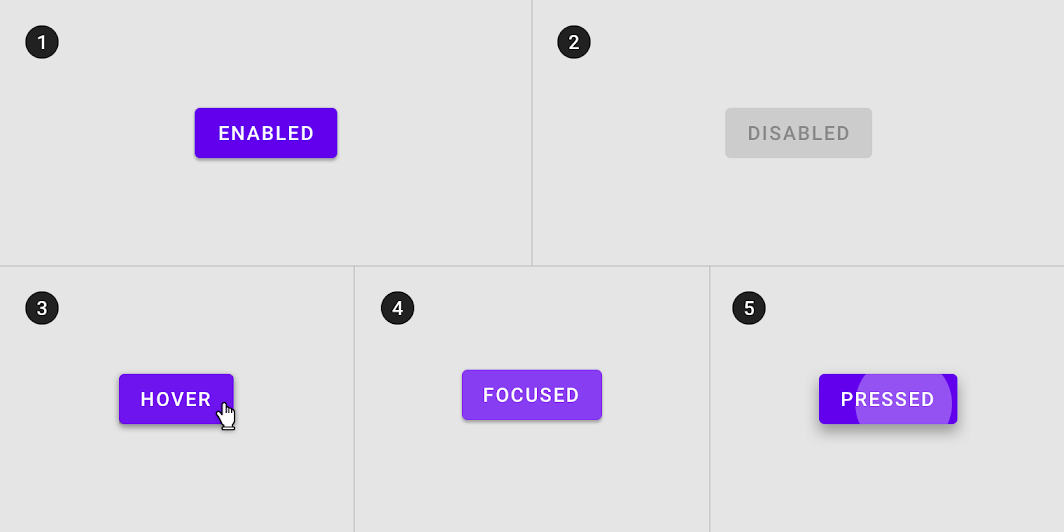
\includegraphics[scale=0.35]{./images/materialUIbutton.png}
    \caption{An example of how a Material UI button varies depending on its state \cite{materialUIbuttons}}
\end{figure}

\subsubsection{Javascript}
Why do we use JS over TS?

\section{Implementation}
This section explores the higher-level design aspects of the web application. We'll discuss the different components that make up the web application in both the UI and the backend.

\begin{figure}[H]
    \centering
    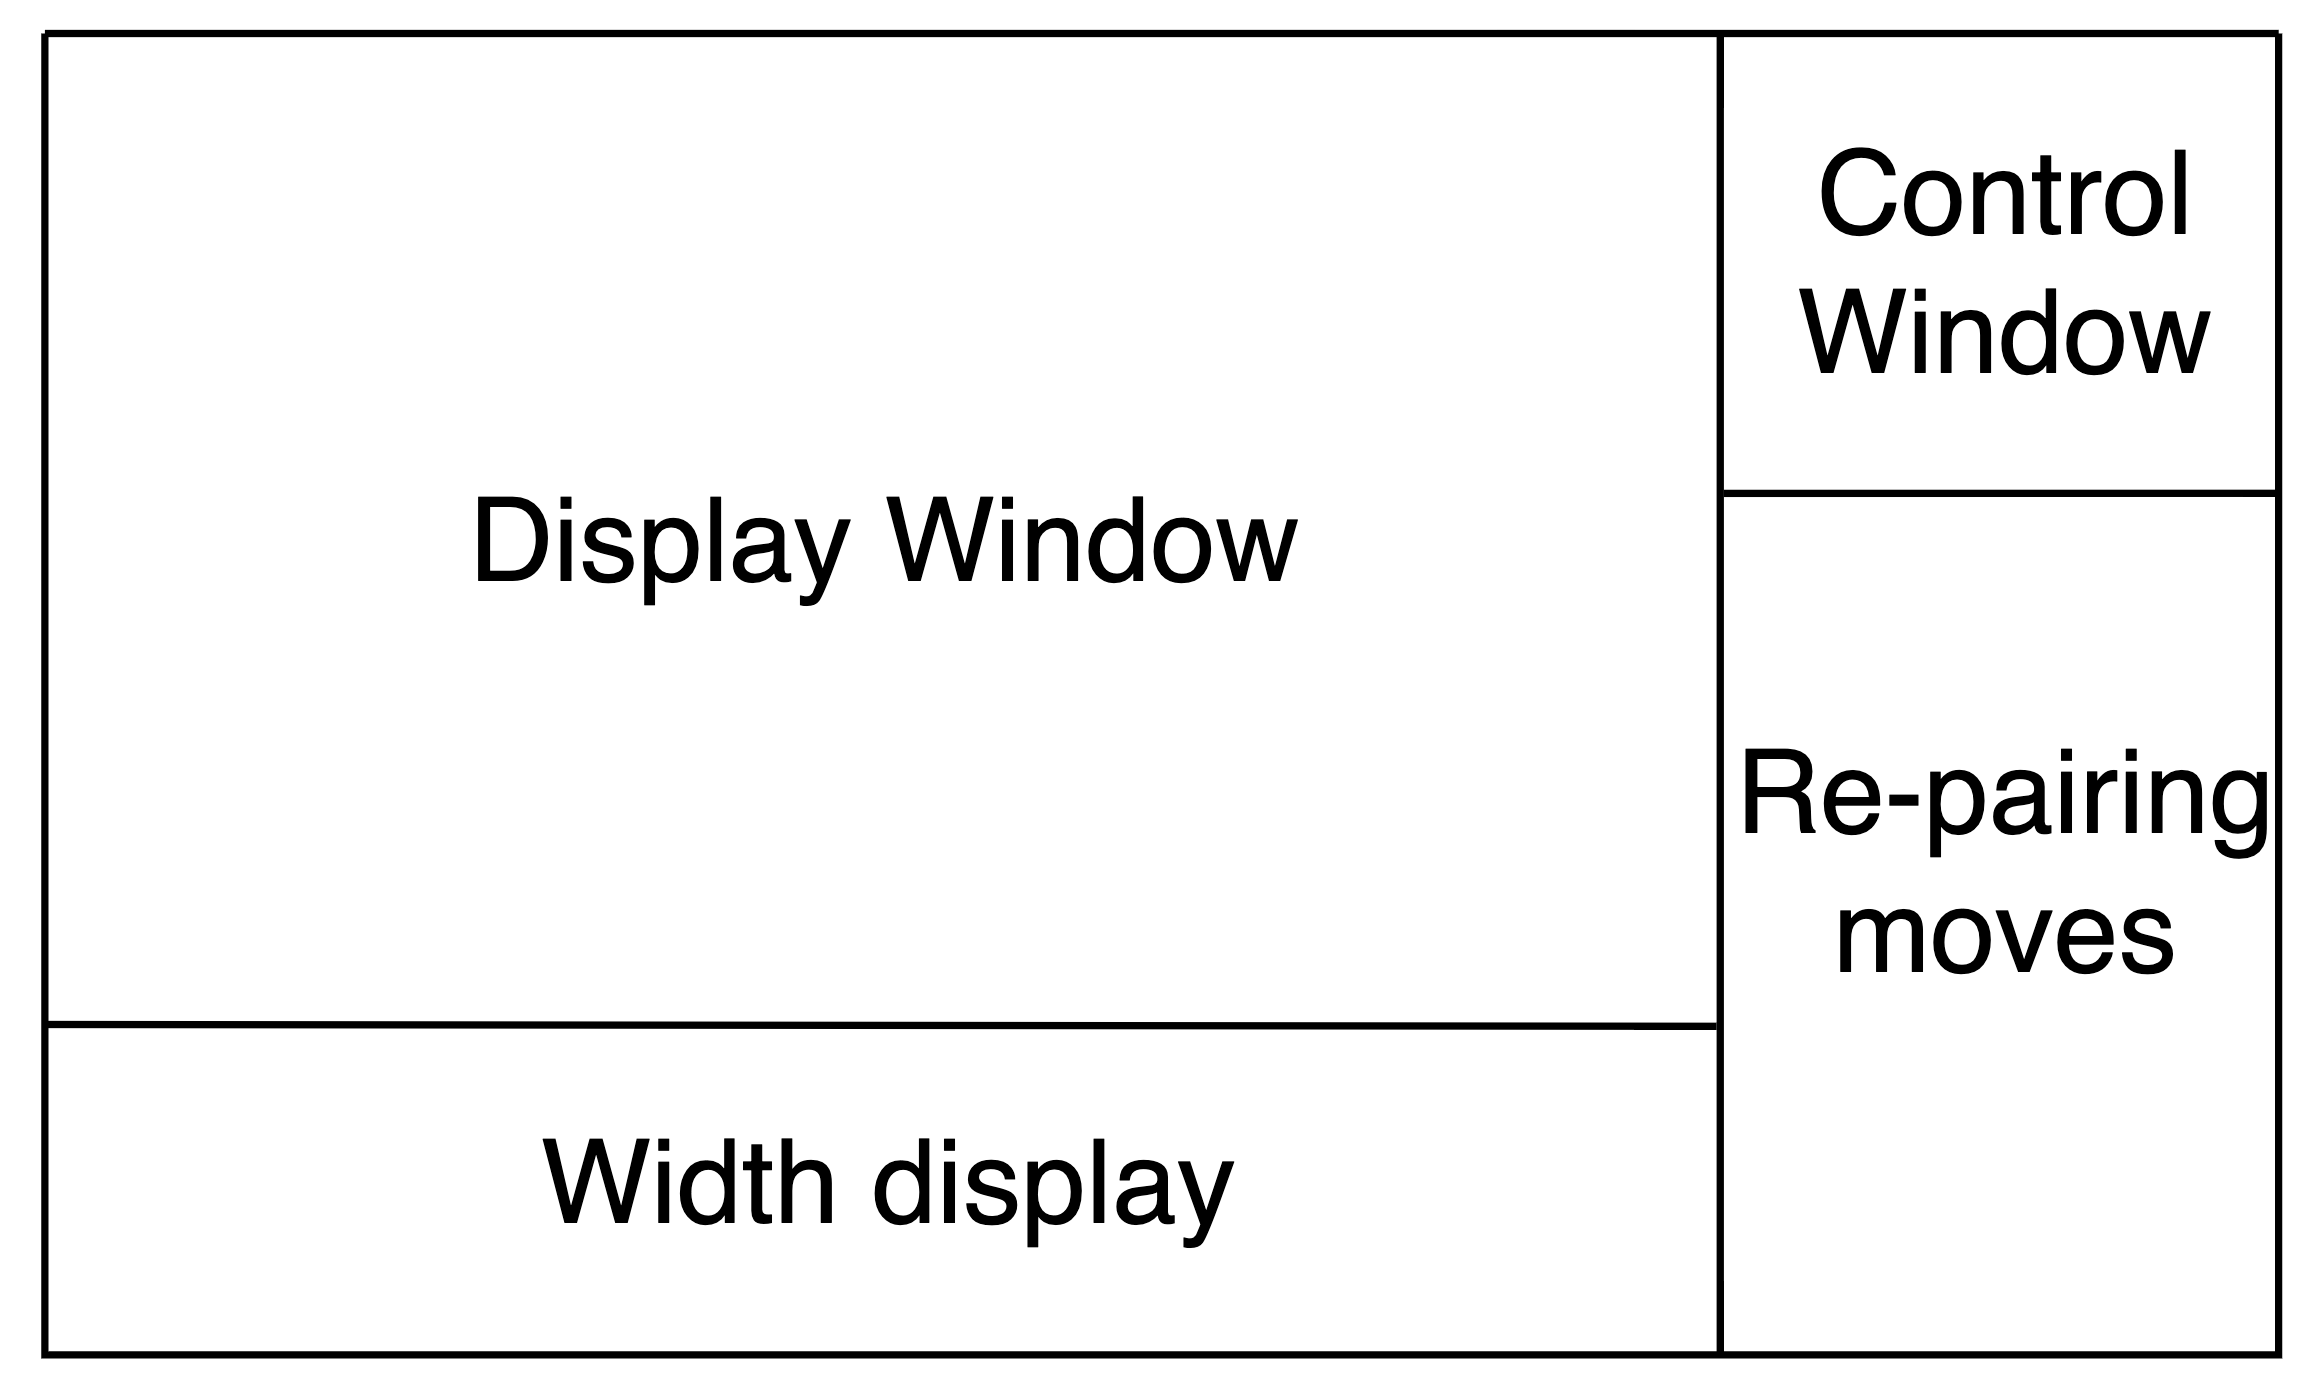
\includegraphics[scale=0.1]{./figures/webBreakdown.png}
    \caption{A high-level overview of the components that make up the web application}
\end{figure}

\subsection{Control Window}
This is where all input and controls will exist. Here the Dyck word will be taken in as input, and all options for runnings strategies

\chapter{Project Management}

\section{Methodology}

\subsection{Development Methodology}
This project used the Agile methodology, as the goals and limitations of the project aligned closely with the principles of Agile \cite{agilePrinciples}:
\begin{itemize}
    \item Creating functional software was of a higher priority than comprehensive documentation. The faster that the software was made functional, the more time could be devoted to its refinement. Given that the author was also new to writing web applications and many of the libraries chosen at the start of this project, making such refinements proved to have a steeper learning curve.
    \item Responding to changes in requirements was of a higher priority than a strict plan and implementation. Throughout the process of absorbing the seminal work \cite{chistikov2020re}, more elegant and useful ideas arose and became the clear option to implement over the current option.
\end{itemize}

% With the initial approach of a local Python app in mind, we begun with writing the strategies as algorithms in Python. However, when the approach was changed 

Note that the \hyperref[softwareReqs]{software requirements} were written in such a way that each one could mostly be handled sequentially, without needing anything that hadn't been met yet. This is roughly the approach taken during development and testing. 

\subsection{Testing Methodology}
As development was done in an Agile manner, it made sense for all testing to be manual, since the functionality of the software was rapidly changing as it was being developed. This meant writing automated tests each time new functionality was required would have been more time-consuming than manual tests. The theoretical nature of the game for which the web application was designed also made manual testing a suitable option; as long as definitions were translated correctly into code and certain edge cases were verified, the software could be expected to perform as required.

All testing was done using a combination of unit testing, incremental integration testing, and requirement-based testing. We elaborate on this process below:

\subsubsection{Unit Testing}
During the development, each of the \hyperref[softwareReqs]{software requirements} was decomposed into smaller functions and subgoals needed to fulfill their relevant requirements. This naturally leads into unit testing; we treated each function as its own unit, and tested it according to the expected functionality. 

For example, to ensure a Dyck word is valid and provide error messages if necessary, we break this down into multiple units as follows:
\begin{enumerate}
    \item A function for the frontend to call and receive data from
    \item A function to check the input against the \hyperref[def:seqDyck]{definition of a Dyck word}, and return a yes or no answer along with a relevant error message
    \item Logic to check if an error was returned
    \item Logic to display the error or the input depending on the result
\end{enumerate}

We then write a function (or in some cases with the frontend, a portion of code or a new state variable) and test each of them work as expected. 

As previously mentioned, by using Flask as the framework of choice for the backend, the Python code required minimal modification to allow functions to serve requests. This made unit testing much easier to perform. 

\subsubsection{Incremental Testing}
After
\section{Setup and Tooling}

\chapter{Project Management}

\section{Methodology}

\subsection{Development Methodology}
This project used the Agile methodology, as the goals and limitations of the project aligned closely with the principles of Agile \cite{agilePrinciples}:
\begin{itemize}
    \item Creating functional software was of a higher priority than comprehensive documentation. The faster that the software was made functional, the more time could be devoted to its refinement. Given that the author was also new to writing web applications and many of the libraries chosen at the start of this project, making such refinements proved to have a steeper learning curve.
    \item Responding to changes in requirements was of a higher priority than a strict plan and implementation. Throughout the process of absorbing the seminal work \cite{chistikov2020re}, more elegant and useful ideas arose and became the clear option to implement over the current option.
\end{itemize}

% With the initial approach of a local Python app in mind, we begun with writing the strategies as algorithms in Python. However, when the approach was changed 

Note that the \hyperref[softwareReqs]{software requirements} were written in such a way that each one could mostly be handled sequentially, without needing anything that hadn't been met yet. This is roughly the approach taken during development and testing. 

\subsection{Testing Methodology}
As development was done in an Agile manner, it made sense for all testing to be manual, since the functionality of the software was rapidly changing as it was being developed. This meant writing automated tests each time new functionality was required would have been more time-consuming than manual tests. The theoretical nature of the game for which the web application was designed also made manual testing a suitable option; as long as definitions were translated correctly into code and certain edge cases were verified, the software could be expected to perform as required.

All testing was done using a combination of unit testing, incremental integration testing, and requirement-based testing. We elaborate on this process below:

\subsubsection{Unit Testing}
During the development, each of the \hyperref[softwareReqs]{software requirements} was decomposed into smaller functions and subgoals needed to fulfill their relevant requirements. This naturally leads into unit testing; we treated each function as its own unit, and tested it according to the expected functionality. 

For example, to ensure a Dyck word is valid and provide error messages if necessary, we break this down into multiple units as follows:
\begin{enumerate}
    \item A function for the frontend to call and receive data from
    \item A function to check the input against the \hyperref[def:seqDyck]{definition of a Dyck word}, and return a yes or no answer along with a relevant error message
    \item Logic to check if an error was returned
    \item Logic to display the error or the input depending on the result
\end{enumerate}

We then write a function (or in some cases with the frontend, a portion of code or a new state variable) and test each of them work as expected. 

As previously mentioned, by using Flask as the framework of choice for the backend, the Python code required minimal modification to allow functions to serve requests. This made unit testing much easier to perform. 

\subsubsection{Incremental Testing}
After
\section{Setup and Tooling}


\clearpage
\emergencystretch=1em
\printbibliography
\end{document}

